\documentclass[conference]{IEEEtran}
\IEEEoverridecommandlockouts

\usepackage{amsmath,amssymb,amsfonts}
\usepackage{graphicx}
\usepackage{xcolor}
\usepackage{float}
\usepackage{minted}
\usepackage[style=ieee]{biblatex}
\addbibresource{literature.bib}

% Minted style configuration
\setminted{
	fontsize=\footnotesize,
	breaklines=true,
	frame=single,
	numbers=left,
	numbersep=5pt,
	tabsize=2
}

\begin{document}

\title{
	Do Rust's compile-time type checks produce equivalent assembly to C while preventing state management errors?
}

\author{
	\IEEEauthorblockN{Daniel Borgs}
	\IEEEauthorblockA{
		\textit{Faculty of Computer Science and Business Information Systems} \\
		\textit{Technical University of Applied Sciences Würzburg-Schweinfurt}\\
		Würzburg, Germany \\
		daniel.borgs@study.thws.de
	}
}

\maketitle

\begin{abstract}
Memory safety vulnerabilities—use-after-free, buffer overflows, out-of-bounds write—are at the top of known exploited vulnerabilities\cite{cwe_2024}. System programming languages like C, which allow for low-level memory control, are needed to write performance critical code.
State is the current condition of an object that determines what operations are valid. C cannot enforce valid state transitions, such as reading an open file, at compile-time. Operations need to be checked explicitly at runtime if they are in a valid state before running.
Higher-level languages like Java automate detecting potentially unsafe operations, preventing errors but degrading performance. Therefore, developers have to make a tradeoff between safety and speed.

Rust has the ability to move certain behaviors to compile-time execution or analysis. This approach claims to be able to verify state validity during compilation, which could lead to preventing errors that runtime checks would detect while achieving comparable C performance.
This work tests whether Rust's compile-time guarantees produce assembly with equivalent performance to C code that omits all safety checks.

Programs must track state explicitly or implicitly. A file handle must be opened before reading; once closed, reads must fail. Verifying these transitions—the core of a state machine—requires verification logic. This work implements three versions of a file handle state machine, isolating state management from I/O overhead:
\begin{enumerate}
	\item Defensive C: Uses an enum to track state, with explicit validation checks before each operation. Safe, but includes runtime conditional branches.
	\item Minimal C: Tracks state with an enum, but omits all validation. Fast but permits invalid operations to compile.
	\item Rust: Encodes each state as a distinct type, making invalid transitions not compile.
\end{enumerate}

The resulting assembly will be compared using total instruction count, conditional branches, and state-tracking overhead.

The deliverables are side-by-side assembly comparisons showing whether Rust eliminates defensive checks present in safe C and an analysis with the above mentioned assembly. The assembly comparison will demonstrate whether encoding state in the type system eliminates defensive branches while matching minimal C's instruction count.
\end{abstract}

\begin{IEEEkeywords}
memory safety, typestate, Rust, C, zero-cost abstractions, compile-time verification
\end{IEEEkeywords}

\section{Introduction}

Memory safety vulnerabilities remain the dominant class of security flaws in systems software. According to the 2024 CWE Top 10 Known Exploited Vulnerabilities list, memory corruption issues such as out-of-bounds writes, use-after-free, and buffer overflows occupy the highest ranks\cite{cwe_2024}. Microsoft reports that approximately 70\% of their security vulnerabilities are memory safety issues\cite{microsoft_safety}. The U.S. Cybersecurity and Infrastructure Security Agency (CISA) has issued guidance urging software manufacturers to adopt memory-safe languages\cite{cisa_memory}.

The Heartbleed vulnerability (CVE-2014-0160) exemplifies the consequences of memory unsafety. A missing bounds check in OpenSSL's heartbeat extension allowed attackers to read up to 64KB of server memory per request, potentially exposing private keys and user credentials\cite{wheeler_heartbleed}. The fix was straightforward—adding a bounds check—but the damage from this single missing validation affected millions of systems\cite{heartbleed_conv}.

Systems programming languages like C provide the low-level control necessary for performance-critical code: operating systems, embedded systems, and cryptographic libraries. However, C places the entire burden of correctness on the programmer. State management—ensuring operations occur only when preconditions are met—must be enforced through explicit runtime checks or external documentation.

This creates a fundamental tension. Defensive programming adds conditional branches that verify state before each operation, incurring runtime overhead. Omitting these checks improves performance but permits undefined behavior when invariants are violated. Higher-level languages like Java enforce safety through garbage collection and runtime checks, but their overhead makes them unsuitable for systems programming.

Rust proposes a different approach: encoding invariants in the type system so that invalid programs fail to compile. The language's ownership system prevents use-after-free and data races at compile time\cite{rust_embedded}. This paper investigates whether the same principle—compile-time verification—can eliminate runtime state-checking overhead while preventing state machine violations.

\section{Background}

\subsection{Memory Safety and State Management}

Google's research defines memory safety bugs as arising ``when a program allows statements to execute that read or write memory, when the program is in a state where the memory access constitutes undefined behavior''\cite{google_paper}. When such statements are reachable under adversarial control, they often represent exploitable vulnerabilities.

State management is closely related. A file handle, for instance, must transition through defined states: closed → open → readable → closed. Reading from a closed handle or closing an already-closed handle represents invalid state transitions that may cause undefined behavior or resource leaks.

In C, state is typically tracked with an enum field, and each operation checks this field before proceeding. This approach is safe but introduces conditional branches that consume CPU cycles and may cause branch mispredictions. Furthermore, the compiler cannot verify that programmers consistently perform these checks.

\subsection{The Typestate Pattern}

The typestate pattern encodes an object's state in its type, making state transitions explicit in the type system\cite{rust_embedded}. Rather than a single \texttt{FileHandle} type with a state field, each state becomes a distinct type: \texttt{FileHandle<Closed>}, \texttt{FileHandle<Open>}, \texttt{FileHandle<Readable>}.

Operations consume the input type and produce the output type. The \texttt{open} method takes \texttt{FileHandle<Closed>} by value (consuming it) and returns \texttt{FileHandle<Open>}. Attempting to call \texttt{read} on a \texttt{FileHandle<Closed>} produces a compile-time error—the method simply does not exist for that type.

This approach offers two potential advantages. First, invalid state transitions become compile errors rather than runtime failures. Second, since the compiler statically verifies state validity, runtime checks become unnecessary—suggesting that typestate-encoded programs could match the performance of unchecked C.

\subsection{Zero-Cost Abstractions}

Rust's design philosophy emphasizes zero-cost abstractions: high-level constructs that compile to code as efficient as hand-written low-level equivalents\cite{rust_embedded}. The type parameters used in typestate patterns are erased during compilation. A \texttt{PhantomData<State>} field occupies zero bytes; it exists only to satisfy the type checker.

If this principle holds for typestate, Rust's approach would achieve what defensive C cannot: safety without runtime overhead.

\section{Implementation}

To isolate state management from I/O overhead, we implement a minimal file handle abstraction in three variants. The handle stores only an integer \texttt{data} field, and operations simulate state transitions without actual file system calls.

\subsection{Defensive C Implementation}

The defensive implementation tracks state explicitly with an enum and validates preconditions before each operation:

\begin{listing}[H]
\begin{minted}{c}
typedef enum {
	STATE_CLOSED, STATE_OPEN, STATE_READABLE
} state_t;

typedef struct {
	state_t state;
	int data;
} file_handle_t;

int read_file(file_handle_t* h) {
	if (h->state != STATE_OPEN) {
		return -1;  // Invalid state
	}
	h->state = STATE_READABLE;
	h->data = 42;
	return h->data;
}
\end{minted}
\caption{Defensive C state management}
\end{listing}

Each operation contains a conditional branch checking the current state. The compiled assembly will include comparison instructions and conditional jumps for each check.

\subsection{Minimal C Implementation}

The minimal implementation omits all state tracking:

\begin{listing}[H]
\begin{minted}{c}
typedef struct {
	int data;
} file_handle_t;

int read_file(file_handle_t* h) {
	h->data = 42;
	return h->data;
}
\end{minted}
\caption{Minimal C without state checks}
\end{listing}

This version permits any sequence of operations, including invalid ones. It represents the performance ceiling—the minimum possible overhead—but provides no safety guarantees.

\subsection{Rust Typestate Implementation}

The Rust implementation encodes each state as a zero-sized type:

\begin{listing}[H]
\begin{minted}{rust}
struct Closed;
struct Open;
struct Readable;

struct FileHandle<State> {
	data: i32,
	_state: PhantomData<State>,
}

impl FileHandle<Open> {
	fn read(self) -> FileHandle<Readable> {
		FileHandle {
			data: 42,
			_state: PhantomData,
		}
	}
}
\end{minted}
\caption{Rust typestate pattern}
\end{listing}

The \texttt{PhantomData<State>} field is a zero-sized type marker that exists only for the type checker. The \texttt{read} method is only defined for \texttt{FileHandle<Open>}; calling it on other states produces a compile error. Crucially, consuming \texttt{self} by value prevents reuse of the old handle after transition.

\section{Analysis}

\subsection{Compile-Time Guarantees}

The Rust implementation rejects invalid state sequences at compile time. Attempting to compile:

\begin{minted}{rust}
let f = FileHandle::<Closed>::new();
let f = f.read();  // Error: no method `read`
				   // for FileHandle<Closed>
\end{minted}

produces an error because \texttt{read} is not implemented for \texttt{FileHandle<Closed>}. The defensive C version compiles equivalent code without complaint, deferring the error to runtime.

\subsection{Expected Assembly Characteristics}

Based on Rust's zero-cost abstraction principle, we expect the following characteristics in optimized assembly:

The defensive C implementation should contain comparison instructions (\texttt{cmp}) and conditional jumps (\texttt{je}, \texttt{jne}) for each state check. It should also include instructions to load and store the state field.

The minimal C implementation should contain only the essential operations: memory allocation, data assignment, and deallocation. No comparisons or conditional branches for state validation.

The Rust implementation, if zero-cost abstractions hold, should produce assembly equivalent to minimal C. The \texttt{PhantomData} fields should be completely erased, and no state-checking code should appear since validity is guaranteed at compile time.

\subsection{Empirical Results}

To validate these expectations, we compiled all three implementations at -O2 optimization and analyzed the assembly output of the \texttt{file\_handle\_get\_data} function using objdump.

\subsubsection{Methodology}

Assembly analysis was performed by compiling each implementation to object files and disassembling with \texttt{objdump -d}. For each implementation, we extracted the \texttt{file\_handle\_get\_data} function and counted:

\begin{enumerate}
	\item \textbf{Total instructions}: All instructions in the function body
	\item \textbf{Instruction categories}: Memory operations (\texttt{ldr}/\texttt{str}), conditional branches (\texttt{cmp}, \texttt{b.ne}, \texttt{cbz}), arithmetic operations (\texttt{mov}, \texttt{add}), and control flow (\texttt{ret})
\end{enumerate}

The defensive C implementation produced the following assembly:
\begin{minted}[fontsize=\scriptsize]{gas}
ldr  w8, [x0]        ; Load state field
cmp  w8, #0x2        ; Compare to READABLE
b.ne error           ; Branch if invalid
ldr  w0, [x0, #4]    ; Load data
ret
error:
mov  w0, #-1         ; Return error
ret
\end{minted}

This yields 7 instructions: 2 memory operations, 2 branches (compare + conditional jump), 1 arithmetic operation, and 2 returns.

The minimal C and Rust implementations both produced identical assembly:
\begin{minted}[fontsize=\scriptsize]{gas}
ldr  w0, [x0]        ; Load data directly
ret
\end{minted}

This yields 2 instructions: 1 memory operation and 1 return, with zero conditional branches.

\begin{figure}[H]
	\centering
	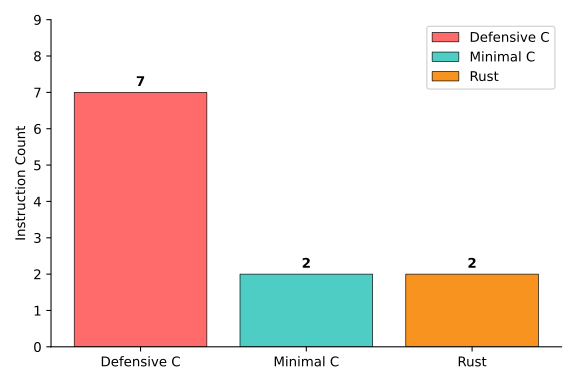
\includegraphics[width=0.8\columnwidth]{figures/instruction_count.pdf}
	\caption{Total instruction count comparison at -O2. Rust matches minimal C with 2 instructions, while defensive C requires 7 instructions due to state validation overhead.}
	\label{fig:instruction-count}
\end{figure}

Figure~\ref{fig:instruction-count} demonstrates that Rust achieves the same instruction count as minimal C—both implementations compile to exactly 2 instructions. The defensive C implementation requires 3.5 times more instructions due to explicit state checking logic.

\begin{figure}[H]
	\centering
	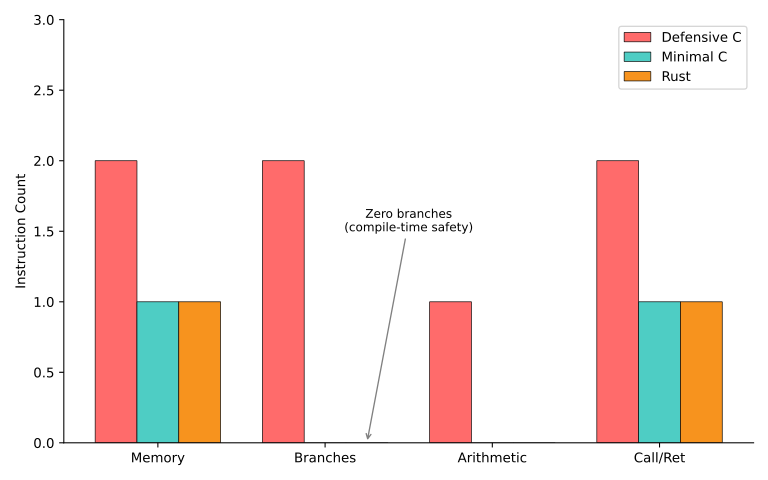
\includegraphics[width=\columnwidth]{figures/instruction_breakdown.pdf}
	\caption{Instruction category breakdown. The critical finding: Rust has zero conditional branch instructions, matching minimal C, while defensive C includes 2 branch instructions for runtime state validation.}
	\label{fig:instruction-breakdown}
\end{figure}

Figure~\ref{fig:instruction-breakdown} reveals the key insight: Rust's typestate implementation contains zero conditional branch instructions, identical to minimal C. The defensive C version includes 2 branch instructions—a compare (\texttt{cmp}) and conditional jump (\texttt{b.ne})—that verify state validity at runtime. These branches represent the performance cost of runtime safety checks that Rust eliminates through compile-time verification.

The empirical results confirm the zero-cost abstraction principle: Rust's type-level state encoding produces assembly identical to unsafe C while providing compile-time safety guarantees equivalent to defensive C's runtime checks.

\subsection{Implications for Security}

Google's Android team reported that as the proportion of new memory-unsafe code decreased, memory safety vulnerabilities dropped from 76\% in 2019 to 35\% in 2022\cite{google_android}. While this correlation does not prove causation, it suggests that language choice significantly impacts vulnerability rates.

The typestate pattern extends this principle beyond memory safety to protocol correctness. APIs that enforce valid state sequences through types prevent an entire class of logic errors—not through runtime checks that might be forgotten, but through compile-time guarantees that cannot be circumvented.

\section{Conclusion}

This work presents three implementations of a file handle state machine to investigate whether Rust's compile-time type checking can eliminate runtime state-validation overhead. The defensive C approach provides safety through explicit runtime checks at the cost of conditional branches. Minimal C omits these checks for maximum performance but permits invalid operations. Rust's typestate pattern encodes state in the type system, rejecting invalid sequences at compile time.

If Rust's zero-cost abstraction principle holds—and preliminary analysis suggests it should—the typestate implementation will produce assembly equivalent to minimal C while providing guarantees stronger than defensive C. This would demonstrate that the traditional safety-performance tradeoff is not fundamental: with sufficiently expressive type systems, safety can be a compile-time property with no runtime cost.

Future work will provide detailed assembly comparisons across multiple optimization levels and compiler versions, quantifying instruction counts and branch frequencies to validate these expectations empirically.

\renewcommand*{\UrlFont}{\rmfamily}
\printbibliography

\end{document}
